\documentclass[10pt,a4paper,english,italian]{article}
\usepackage[T1]{fontenc}
\usepackage[latin1]{inputenc}
\usepackage{babel}
\usepackage{color}
\usepackage{amssymb}
\usepackage{amsmath}
\usepackage{epsfig}
\usepackage{tabularx}
\usepackage{multirow}
\usepackage{subfigure}
\usepackage{verbatim}
\usepackage{babel}
\usepackage{fancyhdr}
\usepackage{listings}
\usepackage{../common/espacs}

\makeatother

%\input{../common/commands.tex}

\title{Esercitazione 5}
\author{D. A. Di Pietro, T. Passerini}

\setlength{\textwidth}{100ex}
\setlength{\oddsidemargin}{0ex}

\pagestyle{fancy}
\headheight 35pt

\rhead{\copyright~Copyright 2006 Daniele A. Di Pietro, Tiziano Passerini}

\begin{document}
\lstset{language=[ISO]C++}
\maketitle

\section*{Descrizione del problema}

L'obiettivo di questa esercitazione \`e implementare le strutture dati
dei lati nella gestione di una \emph{mesh}. \\
Il programma fornito 
gestisce \emph{mesh} bidimensionali costituite da elementi triangolari
e quadrangolari. Per ciascuna forma geometrica sono
fornite funzionalit\`a specifiche, implementate in classi separate. 
La classe \cpp{Mesh} si occupa di memorizzare, in un'opportuna struttura dati,
le informazioni relative alla griglia. 
Tali informazioni sono memorizzate in un file strutturato come segue
\lstset{basicstyle=\scriptsize\sf}
\lstinputlisting[caption=File di esempio contenente la descrizione di
una semplice \emph{mesh}]{./es/2/mesh.msh}
\lstset{basicstyle=\sf}
Si noti che il file d'esempio \`e suddiviso in tre sezioni:
\begin{itemize}
\item la riga successiva all'intestazione \cpp{#DATA} contiene il numero di
nodi e di elementi della griglia;
\item a seguire, l'elenco delle coordinate dei nodi precedute
  dall'intestazione \cpp{#POINTS};
\item in ultimo vi \`e l'elenco degli elementi, caratterizzati dalla
  geometria ($0$ per gli elementi triangolari, $1$ per quelli
  quadrangolari) e dalla sequenza ordinata dei vertici.
\end{itemize}

Poich\`e la classe \cpp{Mesh} contiene elementi di tipo
diverso, sono implementate due classi distinte
\cpp{Triangle} e \cpp{Quadrangle}, che discendono dalla medesima classe
base \cpp{Shape}. Gli elementi della griglia sono memorizzati
utilizzando una lista di puntatori a \cpp{Shape} ed i costrutti per
l'allocazione dinamica. La classe \cpp{Mesh} ha un
costruttore che riceve come argomento il nome di un file di dati di
tipo \cpp{.msh} e costruisce a partire da esso le strutture implementate.

\section*{Es. 1}

Si chiede di implementare i seguenti miglioramenti al codice
\begin{enumerate}
	\item si utilizzi una opportuna struttura dati per contenere i lati della mesh. Inserire
	nella classe \cpp{Mesh} un metodo, di nome \cpp{buildEdges}, che permette di riempire
	tale struttura dati;
	\item si modifichi l'operatore di reindirizzamento ad output della classe \cpp{Mesh}, 
	in modo da riportare a schermo la lista dei lati;
	\item si aggiunga alla classe \cpp{Edge} la possibilit\`a di contenere l'identificativo
	dell'elemento di destra e di sinistra. Si gestisca opportunamente il caso dei lati di bordo.
	\item si modifichi l'operatore di reindirizzamento ad output della classe \cpp{Mesh}, 
	in modo da riportare a schermo anche l'identificativo dell'elemento di destra e di sinistra
	di ciascun lato;
	\item si utilizzi una struttura analoga a quella implementata nel punto 1 per gestire i lati 
	di bordo, senza fare differenza sulla condizione al bordo ad essi associati.
\end{enumerate}

\section*{Es. 2}

Si implementi la possibilit\`a di interrogare la mesh. In particolare si vuole implementare un 
metodo di \cpp{Mesh} che, data una stringa contenente il tipo di condizione di bordo, ritorna
tutti i punti associati. Per risolvere questo punto si utilizzino gli operatori della standard
library.


%Come esercizio aggiuntivo, si scriva una funzione per generare i lati interni e di
%bordo della griglia, memorizzando per ciascuno gli elementi al cui
%bordo appartiene.
%Poich\`e la classe \cpp{Mesh} deve contenere elementi di tipo
%diverso, saranno implementate due classi distinte
%\cpp{Triangle} e \cpp{Quadrangle}, che discendono dalla medesima classe
%base \cpp{Shape}. Gli elementi della griglia saranno quindi memorizzati
%utilizzando una lista di puntatori a \cpp{Shape} ed i costrutti per
%l'allocazione dinamica. La classe \cpp{Mesh} ha un
%costruttore che riceve come argomento il nome di un file di dati di
%tipo \cpp{.msh} e costruisce a partire da esso le strutture richieste.
%
%L'obiettivo di questa esercitazione \`e implementare le strutture dati
%di base per la gestione di una \emph{mesh}. Si supponga di voler
%gestire \emph{mesh} bidimensionali costituite da elementi triangolari
%e quadrangolari. Per ciascuna forma geometrica si vogliono
%fornire funzionalit\`a specifiche, ed \`e, pertanto, prevista 
%un'implementazione con classi separate. Inoltre una classe \cpp{Mesh}
%si occuper\`a di memorizzare in un'opportuna struttura dati
%le informazioni relative alla griglia, che sono memorizzate in un file
%strutturato cos\`i strutturato:
%\lstset{basicstyle=\scriptsize\sf}
%\lstinputlisting[caption=File di esempio contenente la descrizione di
%una semplice \emph{mesh}]{./es/1/mesh.msh}
%\lstset{basicstyle=\sf}
%Si noti che il file d'esempio \`e suddiviso in tre sezioni:
%\begin{itemize}
%\item la riga successiva all'intestazione \cpp{#DATA} contiene il numero di
%nodi e di elementi della griglia;
%\item a seguire, l'elenco delle coordinate dei nodi precedute
%  dall'intestazione \cpp{#POINTS};
%\item in ultimo vi \`e l'elenco degli elementi, caratterizzati dalla
%  geometria ($0$ per gli elementi triangolari, $1$ per quelli
%  quadrangolari) e dalla sequenza ordinata dei vertici.
%\end{itemize}
%
%Poich\`e la classe \cpp{Mesh} deve contenere elementi di tipo
%diverso, saranno implementate due classi distinte
%\cpp{Triangle} e \cpp{Quadrangle}, che discendono dalla medesima classe
%base \cpp{Shape}. Gli elementi della griglia saranno quindi memorizzati
%utilizzando una lista di puntatori a \cpp{Shape} ed i costrutti per
%l'allocazione dinamica. La classe \cpp{Mesh} ha un
%costruttore che riceve come argomento il nome di un file di dati di
%tipo \cpp{.msh} e costruisce a partire da esso le strutture richieste.
%
%\section*{Esercizi con valutazione}
%
%% Completare la libreria proposta con la costruzione della classe \cpp{Edge}. Inoltre
%Svolgere almeno uno dei seguenti esercizi:
%\begin{itemize}
%\item si consideri il caso in cui
%il file di descrizione della mesh contenga anche l'indicazione del
%tipo di condizione al bordo associata a ciascun nodo.
%\lstset{basicstyle=\scriptsize\sf}
%\lstinputlisting[caption=Una semplice \emph{mesh}: sono indicate le
%condizioni al bordo associate ai nodi]{./es/3/mesh.msh}
%\lstset{basicstyle=\sf}
%
%Si utilizzi una opportuna struttura dati per associare
%l'identificativo di ciascun nodo con la stringa che definisce la condizione
%al bordo: si modifichi l'operatore di reindirizzamento ad output della
%classe \cpp{Mesh} per riportare a schermo la condizione al bordo
%associata a ciascun nodo.
%
%Si implementino inoltre le strutture dati e i metodi necessari per
%restituire a schermo una lista di nodi associati ad una certa stringa
%(o un messaggio di avviso se la stringa non \`e associata ad alcun
%nodo).
%
%Per questo esercizio si sfruttino gli algoritmi ed i contenitori STL.
%
%\item Si scriva un metodo della classe \cpp{mesh} che generari tutti i lati della griglia.
%(Suggerimento: per generare i lati, utilizzare il contenitore \cpp{set} o eventualmente \cpp{map} 
% della STL, insieme ad una relazione d'ordine. Memorizzare i lati trovati in un vettore.) 
%\end{itemize}

%Come esercizio aggiuntivo, si scriva una funzione per generare i lati interni e di
%bordo della griglia, memorizzando per ciascuno gli elementi al cui
%bordo appartiene.

%\newpage

\section*{Solutions}

\subsection*{Ex. 1}
This is the required listing
%
\lstset{basicstyle=\scriptsize\sf}
\lstinputlisting{./ex1/sum0.cpp}
\lstset{basicstyle=\sf}
%
Notice that the variable \cpp{temp} is deleted at the end of the \cpp{if} block
inside which it is defined. Similarly the variable \cpp{i} that is used inside
the \cpp{for} loop is not available outside of it. It is common to define the
index of a \cpp{for} loop directly inside the instruction itself like it is done
in the example.

The code can be compiled and executed with the following commands
\begin{verbatim}
g++ -Wall -c sum0.cpp
g++ -o sum0 sum0.o
./sum0
\end{verbatim}
Alternatively the instruction
\begin{verbatim}
g++ -Wall -o sum0 sum0.cpp
\end{verbatim}
compiles the code and performs linking is a single command.
On Unix/Linux systems an executable is not recognized by the extention
\texttt{.exe} like on DOS systems, therefore any extention is suitable, in this
case we chose for an empty one (that is again the common choice).
The parameter \texttt{-Wall} prints to screen almost all the \emph{warnings}.
In this way the compiler reports everything that it finds strange in the code
and that could be the cause of potential errors or problems. It is strongly
adviced to use the flag \texttt{-Wall} every time and read carefully the output.
A good code should not produce any warning at all.

To answer the second point it is sufficient to modify the type of the variable
\cpp{sum} as follows (note that \cpp{0.} is a \emph{floating point} value, while
\cpp{0} is an integer value)
\begin{lstlisting}
int sum = 0;
\end{lstlisting}
The result of the sum of the squares between $1$ and $2000$, stored in
\cpp{sum}, is $-1626300296$. The reason for this misbehavior is due to the fact
that the real value ($2.66867\cdot 10^9$) is above the limit of the storable
values for an integer variable (we triggered an \emph{integer overflow}). In
order to understand why the result is negative, let us consider the case in
which the machine represents an integer with $4$ bytes (e.g.\cpp{sizeof(int)} is
equal to $4$). The biggest positive integer that can be represented is
$2147483647$, with the following binary form
\begin{equation*}
0\quad 1111111~11111111~11111111~11111111
\end{equation*}
where the most significant bit (the leftmost one) is used to set the sign.
Summing $1$ to this value we get
\begin{equation*}
1\quad 0000000~00000000~00000000~00000000
\end{equation*}
that is the representation in two's complement of $-2147483648$, a negative
number. The maximum and minimum value that can be represented for a numeric
type \cpp{T} can be printed to screen using
\begin{lstlisting}
std::cout << std::numeric_limits<T>::max() << " , "
          << std::numeric_limits<T>::min() << std::endl;
\end{lstlisting}
%
\begin{figure}
\centering
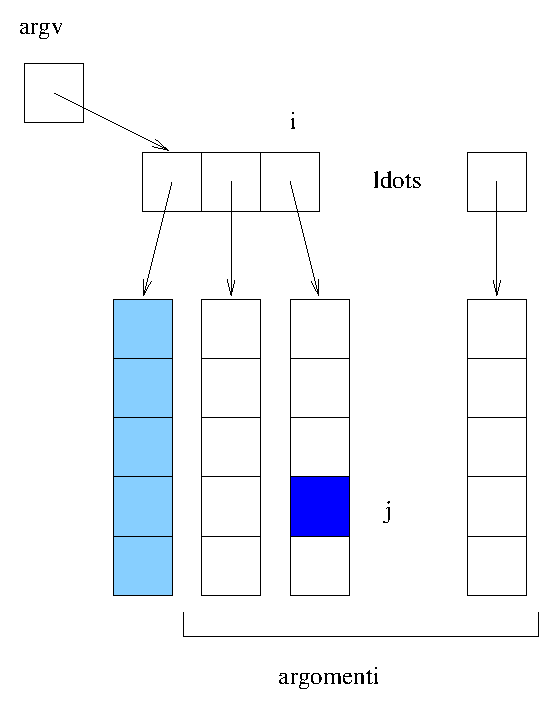
\includegraphics[width=0.4\textwidth]{./figures/tikz/argv}
\caption{\cpp{argv} visual representation. The light blue vector stores the
  name of the executable (in our case it could be \texttt{./sum1}). In blue
  we see the character that corresponds to the call \cpp{argv[i][j]}, where
  \cpp{i} and \cpp{j} are two \cpp{int}.}
\label{fig:argv}
\end{figure}
To answer the third point we use the standard argument for the \cpp{main}
function, \cpp{argc} and \cpp{argv}. The first, \cpp{argc}, is  avariable of
type \cpp{int} that detains the number of arguments that were passed to the
command line. The second, \cpp{argv}, is a vector of c-style character strings,
see \figref{fig:argv}. The first \cpp{argv} element (index $0$) always contains
the executable name, so the parameters are stored starting from index $1$.
Since we are interested in using those parameters as numeric values, we have to
convert the character strings \cpp{argv[1]} and \cpp{argv[2]} to integers. We
can use the function \cpp{atoi} to do it.Note: a vector of character string
pointers can also be interpreted as a matrix of characters, see again 
\figref{fig:argv}.
%
\lstset{basicstyle=\scriptsize\sf}
\lstinputlisting{./ex1/sum1.cpp}
\lstset{basicstyle=\sf}
%
Furthermore, note that the command \cpp{using namespace std} is used to avoid
to specify the qualifier \cpp{std::} to access the objects \cpp{cerr},
\cpp{cout} and \cpp{endl}. The command \cpp{using namespace} must be used with
care, when we are sure that there are no name clashes in the included 
\emph{namespaces}.

\subsection*{Ex. 2}
The listing that is required for the first point is as follows
%
\lstset{basicstyle=\scriptsize\sf}
\lstinputlisting{./ex2/sum1.cpp}
\lstset{basicstyle=\sf}

Note that when we use indices the element numbering in a vector  starts
from $0$ in C++ (as in C). The command \cpp{std::flush} empties the
\emph{output stream buffer}, so the output is phisically performed.
\cpp{std::endl} inserts a \emph{new line} (\cpp{'\n'}) together with a
\cpp{std::flush}.

An alternative way to travel the vector is by using an \emph{iterator}.
Iterators will be throughfully analyzed in the following lessons and are an
extension of the concept of pointer that can be useful to manage standard
library containers. The elements of the vector \cpp{psum} can be printed to
screen using the lines
\lstset{basicstyle=\scriptsize\sf}
\lstinputlisting[linerange={39-41}]{./ex2/sum2.cpp}
\lstset{basicstyle=\sf}

To travel the vector from the last to the first element we can use the
\emph{reverse iterator} of the \cpp{std::vector<double>} type
\lstset{basicstyle=\scriptsize\sf}
\lstinputlisting[linerange={23-24,42-49}]{./ex2/sum3.cpp}
\lstset{basicstyle=\sf}

Note that, differently from the above, a new type psumT has been created with
the command \cpp{typedef}. That type is in fact an \emph{alias} that simplifies
the writing and helps avoiding errors. It becomes usefukl also when there is the
need for a changing the type for the partial sums, since it would be sufficient
to redifine properly the derived type \cpp{psumT}.

The modifications that are required for the third point is implemented in the
following lines that replace the same one in the listing for the first point
\lstset{basicstyle=\scriptsize\sf}
\lstinputlisting[linerange={24-31}]{./ex2/sum2.cpp}
\lstset{basicstyle=\sf}

If the elements were inserted with the \cpp{operator[]} instead of using the
\cpp{push\_back} member at the end the length of the vector would have been
zero (\cpp{psum.size() = 0}) and we would not be able to access the partial
sums. This happens because the \cpp{reserve} member only reserves the memory,
but does not allocate it.

The assignement of the first 10 elements of \cpp{psum} can be performed with
the assign member, that takes as input two iterators that are used as the first
and last location from which to copy
\lstset{basicstyle=\scriptsize\sf}
\lstinputlisting[linerange={51-57}]{./ex2/sum3.cpp}
\lstset{basicstyle=\sf}



\bibliographystyle{siam}
\bibliography{../common/bibliography}

\end{document}
